\subsection{Examples BDD NoSql : }
A l’heure actuelle, il y a plus de 122 solutions NoSQL tous types confondus (Clé/valeur, Document, Colonne et Graphe) sur le marché. La plupart d’entre elles sont soit sous licence Open Source ou soit proposées en SaaS. Les principaux contributeurs (Facebook, Google, Linkedin,…) de ces produits ont développé leurs outils à l’interne avec pour unique but de répondre à leurs propres besoins et non pas dans le but de les commercialiser. Lorsqu’ils se sont trouvés dans un état d’avancement très important (mise en production à l’interne), ces fameux SGBD ont été libérés et mis à disposition du grand public. Il ne faut pas oublier que la fondation Apache joue un grand rôle dans ces divers projets.

On citera quelques-unes classés selon leurs catégories (Pour avoir un plus large aperçu, le site nosql-database.org répertorie tous les produits de type NoSQL):

\subsubsection{BDDs orientés clé-valeur :}

\begin{itemize}[label=\textbullet]
\item \textbf{REDIS}.
\item ORACLE NOSQL.
\item \textbf{VOLDEMORT}.
\item RIAK.
\item INFINISPAN.
\item HAZELCAST.
\end{itemize}

\paragraph{1. Redis:}
Est un projet Open Source de type clé/valeur sous licence BSD. Il dispose de plus de fonctionnalités que la majeure partie des autres solutions du même type. Redis prend en charge certains langages C++, PHP, Ruby,
Python, Perl, Scala, etc. Redis est fait en langage C.

En revanche, un des seuls points négatifs à noter est que Redis ne fournit pas de réel mécanisme de partitionnement, mais uniquement une réplication de type maître/esclave. Malgré cela Redis reste très performant. Il faut aussi ajouter que le projet est sponsorisé par la société VM Ware, ce qui rend la solution crédible et pérenne.

Redis offre les caractéristiques suivantes :
\begin{itemize}[label=\ding{51}]
\item Basculement automatique (sans intervention humaine).
\item Conserve sa base de données entièrement en mémoire.
\item Les transactions sont un moyen d'envoyer en une seule opération un ensemble d'actions.
\item Répliquer les données à un nombre quelconque d'esclaves.
\item Possibilité de contrôler la durée de vie d'une donnée dans la base.
\item Prise en charge de la publication / abonnement.
\end{itemize}
\begin{figure}[h]
	\centering
    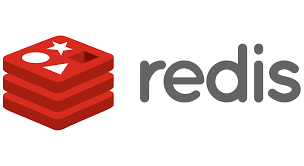
\includegraphics[scale=0.4]{img/4.7}
    \caption{Logo Redis}
\end{figure}
\paragraph{2. Voldemort:}
Est un projet Open Source de type clé/valeur sous licence Apache 2.0. Il a été nommé d’après un personnage du célèbre film « Harry Potter » et offre les caractéristiques suivantes:

\begin{itemize}[label=\ding{51}]
\item Les données sont automatiquement répliquées sur de nombreux serveurs
\item Les données sont automatiquement partitionnées afin que chacun des serveurs obtienne un sous-ensemble d’un ensemble de données
\item L’échec d’un serveur est géré de manière transparente
\item Les données sont « versionnées »
\item Chaque noeud est indépendant des autres. De plus, chaque noeud du système atteint de hauts niveaux de performance de l’ordre des 20Ko d’opérations par seconde.
\end{itemize}

Le projet Voldemort développé par les ingénieurs de LinkedIn a été mis en production à l’interne en 2009. Chez LinkedIn, Voldemort est utilisé pour certaines opérations de stockage de gros volumes de données, ce qui exige des performances accrues auxquelles les solutions de stockage simple ne peuvent répondre.

\begin{figure}[h]
	\centering
    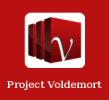
\includegraphics[scale=0.5]{img/4.8}
    \caption{Logo Voldemort}
\end{figure}

\subsubsection{BDDs orientés colonnes :}

\begin{itemize}[label=\textbullet]
\item \textbf{HBASE.}
\item \textbf{CASSANDRA}
\item ACCUMULO.
\item HYPERTABLE.
\end{itemize}

\paragraph{1. HBASE:}
HBase est une base de données distribuée et non relationnelle qui est conçue pour la base de données BigTable par Google. L'un des principaux objectifs de HBase est d'héberger des milliards (de lignes x millions de colonnes). On peut ajouter des serveurs à tout moment pour augmenter la capacité. Et de multiples nœuds maîtres assureront une haute disponibilité des données. Il est composé en Java 8. Il est autorisé sous Apache et est accompagné d'une API Java simple d'utilisation pour l'accès des clients.

Caractéristiques :
\begin{itemize}[label=\ding{51}]
\item Prise en charge de l'échec automatique.
\item Linéairement évolutif.
\item Permet la réplication des données.
\item S'intègre à Hadoop, à la fois comme source et comme destination.
\end{itemize}

\begin{figure}[h]
	\centering
    
\includegraphics[scale=0.4]{img/4.9}
    \caption{Logo HBASE}
\end{figure}

\paragraph{2. CASSANDRA:}
Cassandra est une solution de type orienté colonnes. Mise en Open Source par Facebook en 2008, c’est la fondation Apache qui a repris le flambeau et l’a mise sous licence Apache 2.0. Les caractéristiques de cette solution sont les suivantes:

\begin{itemize}[label=\ding{51}]
\item flexibilité du schéma : chaque « table » est libre de suivre sa propre structure.
\item représentation spatiale de la donnée (cela permet de traiter un grand nombre de lignes)
\item « scalabilité » horizontale : s’il y a besoin de plus de puissance, on rajoute un serveur au cluster.
\item plusieurs niveaux de stratégie de cohérence des données en écriture.
\item réplication multi data-center.
\end{itemize}

Cassandra est utilisée par de nombreux acteurs de premier plan comme Facebook, Twitter et Cisco. Ceci garantit une certaine pérennité du produit. De plus une vaste communauté d’utilisateurs fait partager ses connaissances du produit et le font évoluer.

\begin{figure}[h]
	\centering
    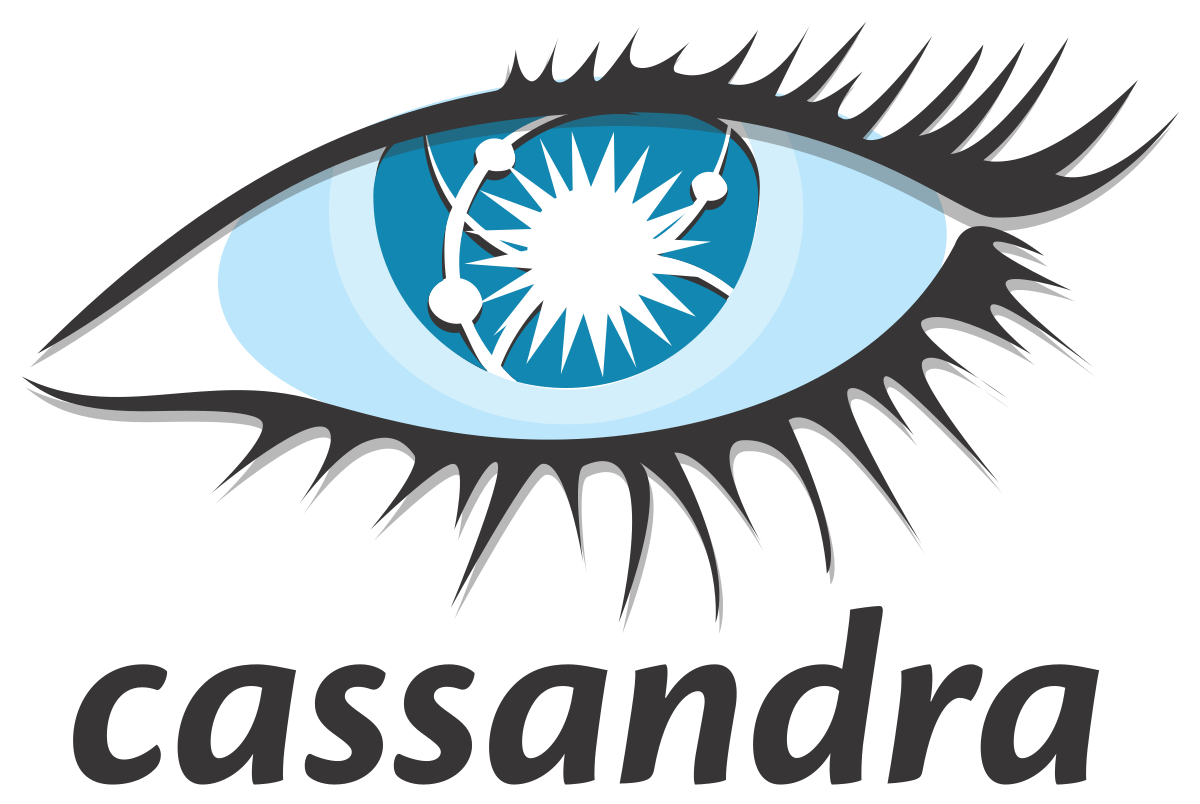
\includegraphics[scale=0.1]{img/4.10}
    \caption{Logo CASSANDRA}
\end{figure}

\subsubsection{BDDs orientés documents :}

\begin{itemize}[label=\textbullet]
\item \textbf{MONGODB.}
\item  \textbf{COUCHDB.}
\item  RAVENDB.
\item  JERRASTORE.
\end{itemize}

\paragraph{1. MONGODB:}
MangoDB est un système de la catégorie orientée documents, le plus populaire de sa catégorie. Il est écrit en C++ et Open Source sous licence AGPL v3.0. Cette solution a été développée par la société 10gen. Voici les caractéristiques du produit:

\begin{itemize}[label=\ding{51}]
\item flexibilité du schéma : chaque document est libre de suivre sa propre structure.
\item format de document JSON.
\item garantit la « scalabilité » horizontale (réplication et « sharding »).
\item support de recherche full-text, géo-spatiale et Map-Reduce.
\item requêtes sur le contenu des documents.
\item une large palette de pilotes est disponible pour divers langages de programmation.
\item bonne documentation.
\end{itemize}

\begin{figure}[h]
	\centering
    
\includegraphics[scale=0.3]{img/4.11}
    \caption{Logo MONGODB}
\end{figure}

\paragraph{2. COUCHDB:}
CouchDB est une base de données NoSQL Open Source qui utilise JSON pour stocker des informations et JavaScript comme langage de requête. CouchDB applique un type de système de contrôle multi-versions pour éviter le blocage du fichier DB pendant l'écriture. C'est autorisé sous Apache. Il est classé 1er sur la liste Best NoSQL Database 2016 pour sa popularité.
Caractéristiques :

\begin{itemize}[label=\ding{51}]
\item Cartographier/réduire la liste et afficher.
\item Assurer la sécurité au niveau de la base de données.
\item L'authentification s'ouvre via un cookie de session comme une application web.
\item JSONP gratuitement.
\item Suivre le stockage des documents.
\item Prise en charge des propriétés ACID.
\item Fournir la forme la plus simple de réplication.
\item Interface utilisateur graphique basée sur un navigateur pour gérer vos données, vos autorisations et votre configuration.
\end{itemize}

\subsubsection{BDDs orientés graphes :}
\begin{itemize}[label=\textbullet]
\item \textbf{Neo4J}
\item INFINATEGRAPHE
\item INFOGRID.
\item HYPERGRAPH DB
\item ALLEGROGRAPH.
\end{itemize}

\paragraph{1. Neo4J:}
Neo4j est un système de base de données orienté graphe. C’est un projet Open Source sous licence GPLv3. Sa première version est sortie en 2007. Ce type de solution est utilisé dans le monde des réseaux sociaux (Ex : amis sur Facebook). Voici quelques caractéristiques du produit :

\begin{itemize}[label=\ding{51}]
\item Transaction complètement ACID.
\item Disponibilité haute.
\item Possibilité d’avoir plus de 64 milliards de noeuds/relations/propriétés sur une JVM.
\item Solution robuste (7ans en production sans interruption).
\item Intégration d’API (librairie Java).
\end{itemize}

Neo Technologie, qui est la société de développement de la base Neo4j, propose un excellent support technique ainsi qu’une documentation complète.

\begin{figure}[h]
	\centering
    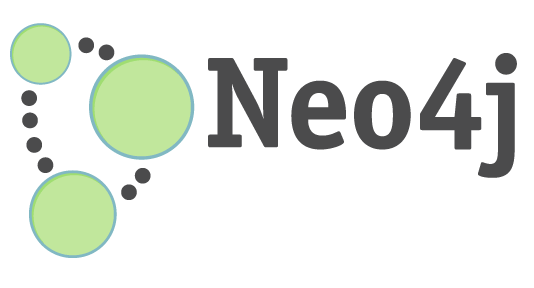
\includegraphics[scale=0.3]{img/4.12}
    \caption{Logo Neo4J}
\end{figure}

\newpage 
\begin{center}
\color[rgb]{0.2, 0.6, 0.2} D'autres base de données peuvent proposées plusieurs services en même temps comme: 
\end{center} 

\paragraph{Amazon DynamoDB:}
DynamoDB utilise un modèle de base de données NoSQL, qui n'est pas relationnel, ce qui permet d'avoir des documents, des graphiques parmi ses modèles de données.  Chaque requête DynamoDB est exécutée par une clé primaire identifiée par l'utilisateur, qui identifie de manière unique chaque élément. Il libère également les clients du fardeau de l'exploitation et de la mise à l'échelle d'une base de données distribuée. Ainsi, le provisionnement matériel, l'installation, la configuration, la réplication, le patch logiciel, la mise à l'échelle des clusters, etc. sont gérés par Amazon.

Caractéristiques :
\begin{itemize}[label=\ding{51}]
\item Haute évolutivité.
\item Plage de hachage pour l'indexation d'une plage de valeurs.
\item Stockage des données dans les partitions.
\item Utilise JSON comme protocole de transport et non comme format de stockage.
\end{itemize}